
\chapter{Connessione degli Host domotici alla VPN \ok \ok}
\label{ch:connessione-host-domotici}

\section{Overview della configurazione \ok}

L'ultima parte della configurazione consiste nel rendere disponibile nella VPN la rete locale del \textit{router 4g}, consentendo quindi lo scambio di dati tra gli \textit{host-domotici} e i \textit{Client} della VPN.

Per fare ciò si dovrà configurare il \textit{Router} in modo che effettui il forwarding verso la VPN, e il \textit{Server} in modo che annunci la sottorete del \textit{Router} a tutti gli Host della VPN.


In fig.~\ref{fig:diag2-host_real} è possibile vedere la configurazione iniziale per questo capitolo, cioè la configurazione finale del capitolo \ref{ch:configurazione-router} con l'aggiunta dell'\textit{host-domotico} connesso al \textit{Router}. 


\begin{figure}[H]
    \centering
    \savebox{\myimage}{
        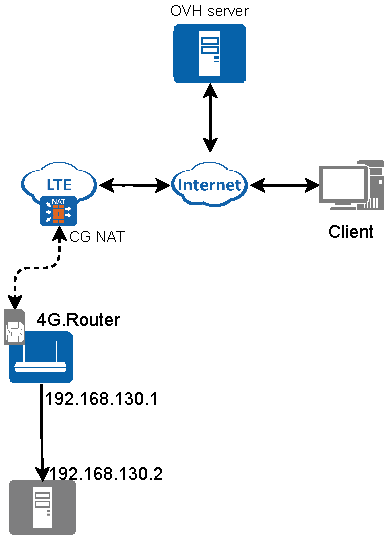
\includegraphics[width=0.44\linewidth]{immagini/diag2-host_real}
    }
    \begin{subfigure}{0.44\linewidth}
        \centering
        \usebox{\myimage}
        \caption{Diagramma reale della configurazione iniziale per questo capitolo}
        \label{fig:diag2-host_real}
    \end{subfigure}
    \hfill
    \begin{subfigure}{0.53\linewidth}
        \centering
        \raisebox{\dimexpr.5\ht\myimage-.6\height\relax}{
            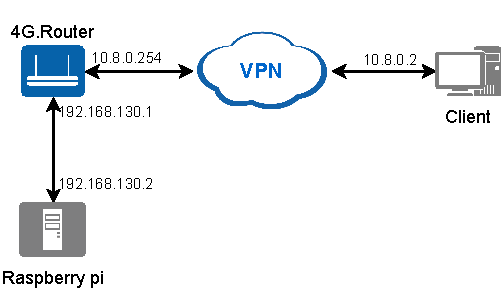
\includegraphics[width=1\linewidth]{immagini/diag2-host_virtual}
        }
        \caption{Diagramma della topologia virtuale finale.\newline}
        \label{fig:diag2-host_virtual}
    \end{subfigure}
    \caption{Schemi concettuali della configurazione iniziale e finale per il capitolo~\ref{ch:connessione-host-domotici}.}
\end{figure}

Una volta conclusa la configurazione si arriverà a una topologia virtuale descritta in fig.~\ref{fig:diag2-host_virtual}, che costituisce inoltre la topologia di obbiettivo per questo elaborato (fig.~\ref{fig:schema_architettura_virtuale}).

\section{Configurazione del firewall nel \textit{Router} \ok}

\subsection{Creazione della zona firewall per la VPN \ok}
\label{subsec:creazione-firewall-zone-vpn}

Per rendere possibile la comunicazione tra la rete \textit{lan} del \textit{Router} e la VPN è necessario configurare opportunamente il firewall nel \textit{Router}.

Ciò viene fatto direttamente da LuCI, nella sezione firewall si avranno preconfigurate delle zone firewall, in questo caso sono presenti di default 2 zone: \textit{lan} e \textit{wan}

\begin{figure}[H]
    \centering
    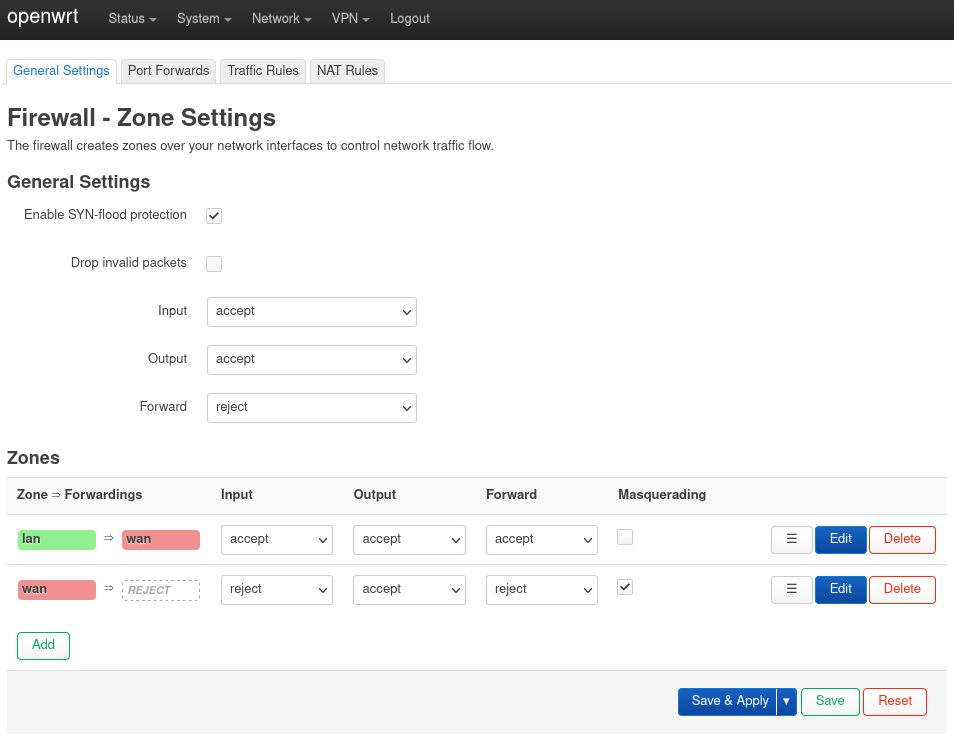
\includegraphics[width=1\linewidth]{immagini/LuCI_firewall_init1}
    \caption{Configurazione di default delle zone del firewall.}
    \label{fig:luci-firewall-init}
\end{figure}

Le 2 zone sono collegate alle relative interfacce: la zona \textit{lan} è collegata all'interfaccia relativa alla rete interna del \textit{Router}; la zona \textit{wan} è collegata all'interfaccia esterna del \textit{Router}. 

\newpage
Si deve quindi aggiungere una nuova zona, chiamata \textit{vpn}, che successivamente sarà collegata all'interfaccia virtuale della VPN (\textit{tun0}). La zona \textit{vpn} dovrà avere le seguenti opzioni:

\begin{itemize}[nosep]
    \item Policy di forward: accept
    \item Forward consentito verso la zona \textit{lan}
    \item Forward consentito dalla zona \textit{lan}
\end{itemize}

In figura \ref{fig:luci-firewall-vpn} è possibile vedere la pagina di configurazione con le opzioni inserite.

\begin{figure}[H]
    \centering
    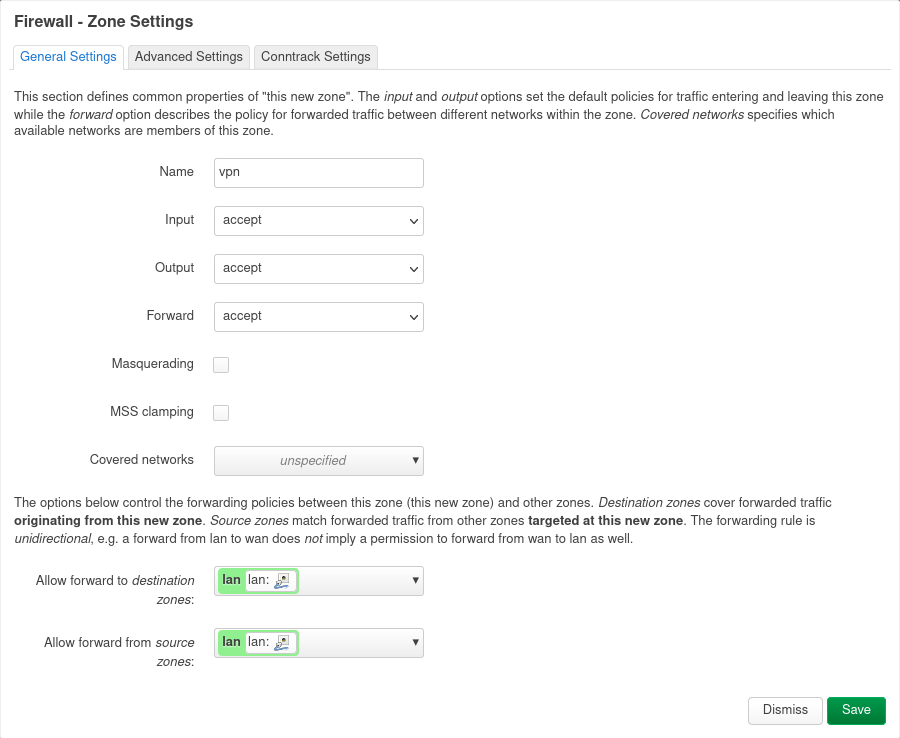
\includegraphics[width=1\linewidth]{immagini/LuCI_firewall_vpn1}
    \caption{Schermata di aggiunta di una nuova zona firewall.}
    \label{fig:luci-firewall-vpn}
\end{figure}

\newpage
Dopo aver salvato, la pagina del firewall sarà:

\begin{figure}[H]
    \centering
    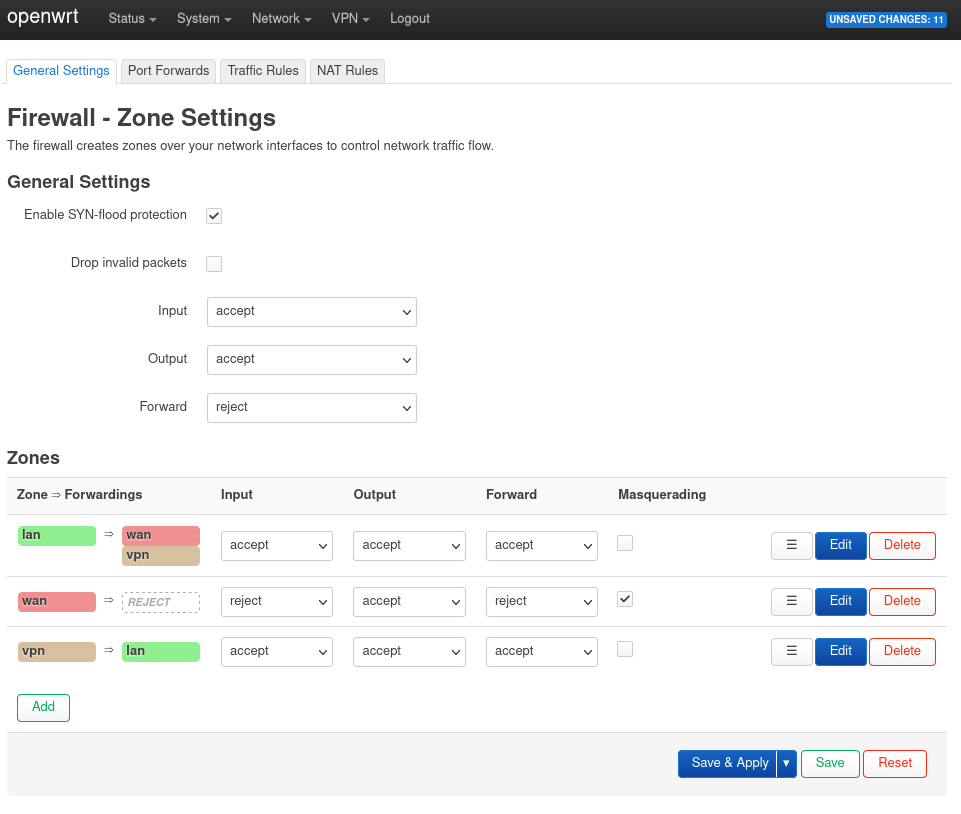
\includegraphics[width=1\linewidth]{immagini/LuCI_firewall_end1}
    \caption{Configurazione delle zone firewall dopo l'aggiunta della zona \textit{vpn}.}
    \label{fig:luci-firewall-end}
\end{figure}

\subsection{Aggiunta dell'interfaccia \textit{tun0} alla zona firewall \textit{vpn} \ok}
\label{subsec:aggiunta-interfaccia-tun0-zona-vpn}

Per far effettivamente funzionare la zona firewall aggiunta nella sezione precedente, si deve aggiungere l'interfaccia relativa alla VPN (\textit{tun0}) alla zona \textit{vpn}.

Dato che l'interfaccia \textit{tun0} non è presente in LuCI, la si deve creare usando le opzioni che già conosciamo. Durante la creazione, nella sezione \textit{Firewall Settings}, sarà possibile assegnare l'interfaccia a una zona firewall.

Quindi nella sezione \textit{interfaces}, si deve aggiungere una nuova interfaccia con le seguenti opzioni:

\begin{itemize}[nosep]
    \item \bf{Name}: tun0
    \item \bf{Proto}: static
    \item \bf{Device}: tun0
    \item \bf{ipv4 address}: 10.8.0.254
    \item \bf{ipv4 netmask}: 255.255.255.0
    \item \bf{Assign firewall zone}: vpn
\end{itemize}

\begin{figure}[H]
    \centering
    \begin{subfigure}{1\linewidth}
        \centering
        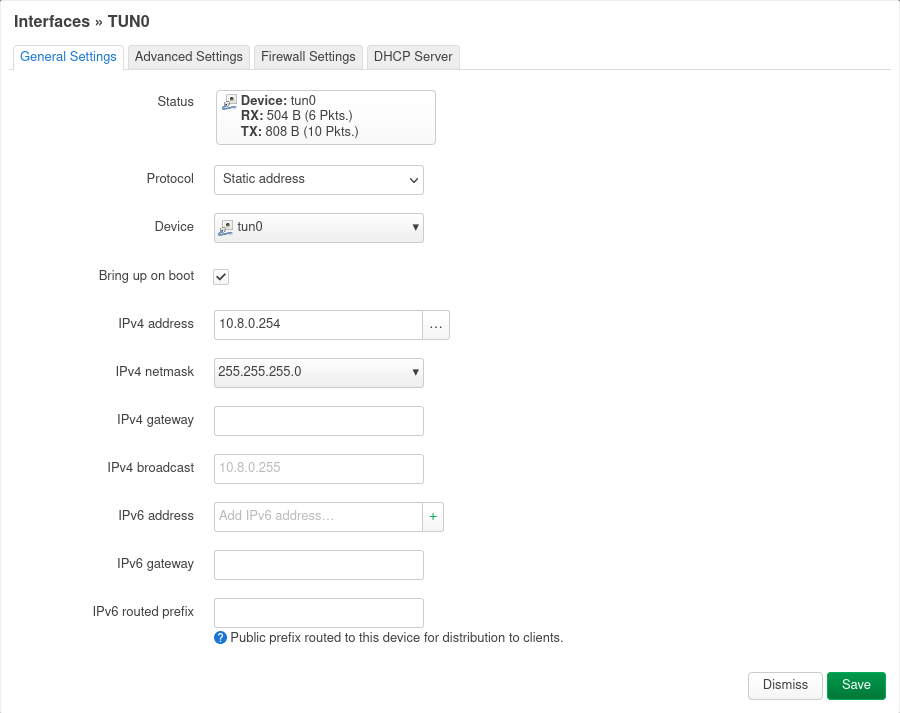
\includegraphics[width=1\linewidth]{immagini/LuCI_int_tun0_1}
        \caption{General settings}
        \label{fig:luci-firewall-interfaces}
    \end{subfigure}
    \medskip
    \begin{subfigure}{1\linewidth}
        \centering
        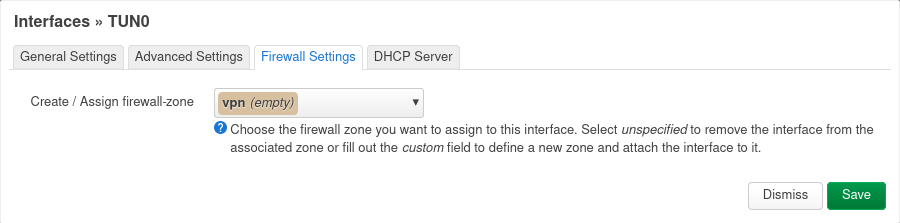
\includegraphics[width=1\linewidth]{immagini/LuCI_int_tun0_2}
        \caption{Firewall settings}
        \label{fig:luci-firewall-interfaces1}
    \end{subfigure}
    \caption{Assegnazione interfaccia \textit{tun0} alla zona firewall \textit{vpn} tramite interfaccia LuCI}
\end{figure}

A questo punto i pacchetti provenienti dalla \it{lan} del \textit{Router} vengono inoltrati correttamente nella VPN, ma gli Host nella VPN non hanno una rotta verso la rete interna del router, perciò la comunicazione risulta ancora mono direzionale. È possibile verificarlo con un semplice test i cui:

\begin{itemize}[nosep]
    \item l'host-domotico effettua il ping verso il client;
    \item il \textit{Router} è in ascolto sull'interfaccia \textit{tun0} con \code{tcpdump};
\end{itemize}

\begin{bashcode}{Host-domotico}{}
$ ping -c1 10.8.0.2     # client 1
PING 10.8.0.2 (10.8.0.2) 56(84) bytes of data.

--- 10.8.0.2 ping statistics ---
1 packets transmitted, 0 received, 100% packet loss, time 0ms
\end{bashcode}

\begin{bashcode}{Router}{}
$ tcpdump -i tun0
15:33:38.363082 IP 192.168.130.2 > 10.8.0.2: ICMP echo request, id 17, seq 1, length 64
\end{bashcode}

Si vede come il pacchetto ICMP \textit{echo request} venga correttamente inoltrato nella VPN dal \textit{Router}, ma il \code{ping} fallisce poiché che non vi è nessun \textit{echo reply} dal \textit{Client}.


\section{Modifiche alla configurazione OpenVPN del \textit{Server} \ok}
\label{sec:hosts-openvpn-server}

Come visto nella sezione precedente, la comunicazione tra \textit{host-domotico} e \textit{Client} è ancora mono direzionale. Per renderla bidirezionale, si deve modificare la configurazione del \textit{Server} di OpenVPN facendo in modo che:

\begin{enumerate}
    \item il \textit{Server OpenVPN} sia consapevole che il \textit{Router} vuole esporre una sua sottorete verso la VPN;
    \item i client della VPN abbiano l'opportuna rotta per raggiungere la sottorete dove si trova l'\textit{host-domotico};
\end{enumerate}


Per il punto 1 è necessario aggiungere l'opzione \code{iroute} \cite{openvpn-iroute} nel file \\\code{/etc/openvpn/server/ccd/router}, creato in sezione \ref{sec:static-ip-router}:

\begin{bashcode}{Server}{}
$ vim /etc/openvpn/server/ccd/router
ifconfig-push 10.8.0.254 255.255.255.0
iroute 192.168.130.0 255.255.255.0      # net e netmask della rete lan del router
\end{bashcode}

Per il punto 2 è necessario usare l'opzione \code{push "route [...]"} \cite{openvpn-push-route} nella configurazione OpenVPN nel \textit{Server}:

\begin{bashcode}{Server}{}
$ vim /etc/openvpn/server/server.conf
168 push "route 192.168.130.0 255.255.255.0"
\end{bashcode}

Dopo aver modificato la configurazione del \textit{Server} è necessario riavviarlo con \\\code{systemctl restart}.

In questo modo nella procedura di connessione alla VPN, i client aggiungeranno la rotta verso la sottorete \code{192.168.130.0/24} nella loro tabella di routing. Possiamo verificarlo con: 

\begin{bashcode}{Client}{}
$ ip route
[...]
192.168.130.0/24 via 10.8.0.1 dev tun0
\end{bashcode}

\section{Test e analisi della configurazione }

Al termine della procedura di configurazione esposta, l'obbiettivo precedentemente fissato in sezione \ref{sec:overview-goal} risulta completamente raggiunto. Ma è opportuno effettuare alcuni test che coprono i casi d'uso più comuni.

Nelle procedure di verifica verranno usate le utility \code{ping}, \code{tracepath} e \code{tcpdump}, poste in vari punti della topologia, in modo da valutare il percorso reale e virtuale dei pacchetti.

Supponendo per esempio che il \textit{Client} voglia comunicare con un \textit{host-domotico}, in questo caso la \textit{Raspberry Pi} che ha IP \code{192.168.130.2}, e che il dato da trasmettere sia un ICMP \textit{echo request}, facente parte di un \code{ping}.

\begin{figure}[H]
    \centering
    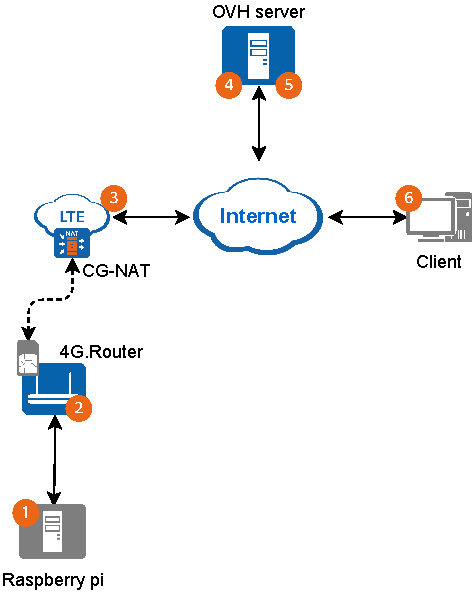
\includegraphics[width=0.5\linewidth]{immagini/diag2-test_real}
    \caption{Topologia finale con evidenziati alcuni punti di interesse nel percorso del pacchetto.}
    \label{fig:diag-test-real}
\end{figure}

\newpage
Nell'analisi andremo a seguire il percorso del pacchetto nei punti di interesse rappresentati in fig.~\ref{fig:diag-test-real}, esaminando in modo dettagliato cosa succede ad ongi step:

\begin{enumerate}
    \item[1.] Il \textit{Client} (\code{10.8.0.2}) effettua il ping verso l'\textit{host-domotico} (\code{192.168.130.2}).
\begin{bashcode}{Client}{}
$ ping -c 1 192.168.130.2
\end{bashcode}
    
    Il \textit{Client} ha la subnet \code{192.168.130.0/24} nella sua tabella di routing (sezione \ref{sec:hosts-openvpn-server}), può essere quindi costruito un pacchetto di tipo ICMP \textit{echo request} che ha come IP sorgente \code{10.8.0.2} e come destinazione \code{192.168.130.2}. 
    
    A questo punto il \textit{Client OpenVPN} lo cifra e incapsula in un ulteriore pacchetto IP (sezione \ref{subsec:openvpn-networking}), che questa volta ha IP di destinazione \code{51.178.141.119}, cioè l'IP pubblico del \textit{Server}. Il pacchetto può essere quindi trasmesso attraverso Internet.
    

    \item[2.] Il \textit{Server} riceve il pacchetto, vedendo che il payload è di tipo OpenVPN lo inoltra al \textit{Server OpenVPN} (sezione \ref{sec:network_stack} e \ref{sec:firewall}). 
    
    Il contenuto del pacchetto viene quindi decifrato e analizzato.
    
    Dato che l'opzione \code{client-to-client} è abilitata (sezione \ref{sec:client-to-client}) il traffico non passa per l'interfaccia \code{tun0}, infatti mettendoci in ascolto con \code{tcpdump} non vediamo nessun pacchetto:
\begin{bashcode}{Server}{}
$ tcpdump -i tun0
\end{bashcode}
    Possiamo però vedere il pacchetto transitare sull'interfaccia esterna del \it{Server} (\it{ens3}). In questo caso però vedremo il pacchetto esterno, possiamo riconoscerlo e distinguerlo dal normale traffico internet selezionando la porta di OpenVPN:
\begin{bashcode}{Server}{}
$ sudo tcpdump -i ens3 -n port 1194
15:43:15.543169 IP 151.57.44.194.59478 > 51.178.141.119.1194: UDP, length 108
\end{bashcode}
    

    \item[3.] Il \textit{Server OpenVPN} analizza il campo IP di destinazione e verifica che il pacchetto è destinato nella subnet \code{192.168.130.0/24}, data la configurazione fatta in sezione \ref{sec:hosts-openvpn-server}, il \textit{Server} provvederà a inoltrarlo al \textit{Router} (\code{10.8.0.254}).
    
    La comunicazione attraverso il NAT è possibile poiché OpenVPN implementa nel suo protocollo una serie di pacchetti \textit{keepalive} \cite{openvpn-keepalive} tra ogni Host e il Server. Ciò permette al NAT di sapere a quale host della sua rete privata deve inoltrare i pacchetti. 
    
    Il pacchetto viene cifrato con il certificato del \it{Router} e inoltrato usando come IP di sorgente \code{51.178.141.119} e destinazione l'IP pubblico del NAT.
    \newpage
    Possiamo vedere il pacchetto in uscita dal \it{server} mettendoci in ascolto sull'interfaccia \it{ens3}:
\begin{bashcode}{Server}{}
$ sudo tcpdump -i ens3 -n port 1194
15:43:15.543273 IP 51.178.141.119.1194 > 151.47.152.251.40637: UDP, length 108
\end{bashcode}


    \item[4.] Il NAT effettua la traduzione, modificando l'IP e la porta del pacchetto esterno e lo inoltra all'interfaccia \textit{wan} del \textit{Router}.
    

    \item[5.] Il \textit{Router} riceve il pacchetto e lo decifra usando il suo certificato. Vedendo che il pacchetto interno è destinato alla subnet \code{192.168.130.0/24}, deve essere quindi inoltrato alla sua \textit{lan} (sezione \ref{subsec:creazione-firewall-zone-vpn} e \ref{subsec:aggiunta-interfaccia-tun0-zona-vpn}). 
    
    Il pacchetto interno viene quindi inoltrato all'\textit{host-domotico} (\code{192.168.130.2}). 
    
    In questo caso è possibile vedere il percorso del pacchetto decifrato con \code{tcpdump}:
\begin{bashcode}{Router}{}
$ tcpdump -i tun0
10:44:07.228387 IP 10.8.0.2 > 192.168.130.2: ICMP echo request, id 12, seq 1, length 64
\end{bashcode}
    
    \item[6.] Il \textit{host-domotico} riceve il pacchetto e legge il contenuto, vedendo che si tratta di ICMP \textit{echo request} provvede a costruire una risposta ICMP \textit{echo reply} e la invia al \textit{Client}. Ciò viene fatto invertendo sorgente e destinazione del pacchetto \it{echo request}, cioè impostando sorgente: \code{192.168.130.2}; e destinazione: \code{10.8.0.2}.

\end{enumerate}


Se è stato configurato tutto correttamente il \code{ping} avrà successo:
\begin{bashcode}{Client}{}
$ ping -c 1 192.168.130.2
PING 192.168.130.2 (192.168.130.2) 56(84) bytes of data.
64 bytes from 192.168.130.2: icmp_seq=1 ttl=63 time=0.643 ms

--- 192.168.130.2 ping statistics ---
1 packets transmitted, 1 received, 0% packet loss, time 0ms
rtt min/avg/max/mdev = 0.643/0.643/0.643/0.000 ms
\end{bashcode}


\begin{comment}
Considerando solo il percorso del pacchetto interno si ha una semplificazione del diagramma~\ref{fig:diag-test-real}:

\begin{figure}[H]
    \centering
    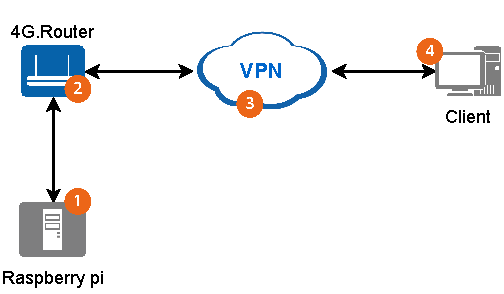
\includegraphics[width=0.5\linewidth]{immagini/diag2-test_virtual}
    \caption{Topologia virtuale finale, con evidenziati i punti di interesse nel percorso del pacchetto.}
    \label{fig:diag-test_virtual}
\end{figure}

\end{comment}

\newpage
È inoltre possibile verificare il percorso del pacchetto interno (cifrato) usando la utility \code{tracepath}, che permette di vedere l'indirizzo IP di tutti i router che sono presenti tra chi esegue il comando e la destinazione:

\begin{bashcode}{Client}{}
$ tracepath 192.168.130.2
1?: [LOCALHOST]                      pmtu 1500
1:  10.8.0.254                       0.471ms
1:  10.8.0.254                       0.473ms
2:  192.168.130.2                    0.567ms reached
    Resume: pmtu 1500 hops 2 back 2
\end{bashcode}

Come era previsto l'unico router presente nella topologia virtuale è il \it{Router 4G} (\code{10.8.0.254}).


Con questi test possiamo concludere che la topologia sia stata implementata correttamente.

\begin{comment}



\begin{bashcode}{Client}{}
$ ping -c 1 192.168.130.2
PING 192.168.130.2 (192.168.130.2) 56(84) bytes of data.
64 bytes from 192.168.130.2: icmp_seq=1 ttl=63 time=0.643 ms

--- 192.168.130.2 ping statistics ---
1 packets transmitted, 1 received, 0% packet loss, time 0ms
rtt min/avg/max/mdev = 0.643/0.643/0.643/0.000 ms
\end{bashcode}


\begin{bashcode}{Host-domotico}{}
$ ping -c 1 10.8.0.2
PING 10.8.0.2 (10.8.0.2) 56(84) bytes of data.
64 bytes from 10.8.0.2: icmp_seq=1 ttl=63 time=0.428 ms

--- 10.8.0.2 ping statistics ---
1 packets transmitted, 1 received, 0% packet loss, time 0ms
rtt min/avg/max/mdev = 0.428/0.428/0.428/0.000 ms
\end{bashcode}

\begin{bashcode}{Router}{}
$ tcpdump -i tun0
listening on tun0, link-type RAW (Raw IP), capture size 262144 bytes
11:56:10.469901 IP 192.168.130.2 > 10.8.0.2: ICMP echo request, id 14, seq 1, length 64
11:56:10.470230 IP 10.8.0.2 > 192.168.130.2: ICMP echo reply, id 14, seq 1, length 64
\end{bashcode}


\begin{bashcode}{Client}{}
$ tracepath 192.168.130.2
1?: [LOCALHOST]                      pmtu 1500
1:  10.8.0.254                       0.471ms
1:  10.8.0.254                       0.473ms
2:  192.168.130.2                    0.567ms reached
    Resume: pmtu 1500 hops 2 back 2
\end{bashcode}

\begin{bashcode}{host-domotico}{}
$ tracepath 10.8.0.2
1?: [LOCALHOST]                      pmtu 1500
1:  router-1                         0.062ms
1:  router-1                         0.068ms
2:  10.8.0.2                         0.592ms reached
    Resume: pmtu 1500 hops 2 back 2
\end{bashcode}

\end{comment}

